\documentclass[12pt, a4paper]{article}
\usepackage[margin = 1in, top=1.3in]{geometry}
\usepackage[english]{babel}
\usepackage[utf8]{inputenc}
\usepackage{fancyhdr}
\usepackage[fleqn]{amsmath}
\usepackage{mathtools}
\usepackage{tabto}
\usepackage{bm}
\usepackage{graphicx}
\graphicspath{{./images/}}
\usepackage[font=small,labelfont=bf]{caption}
 
\pagestyle{fancy}
\fancyhf{}
\rhead{\small{Shaan Ul Haque(180070053)\\ Samarth Singh (180050090) \\ Niraj Mahajan (180050069)}}
\lhead{CS-663 Assignment-4 : Question 4}
\rfoot{Page 4.\thepage}
 
\begin{document}
\vspace*{-22pt}
\section*{Question 4}
\subsection*{4.1: Results on the ORL datset}
\subsubsection*{PCA using SVD}
\quad In this section, we performed PCA by performing SVD of the $X_{dxn}$ data matrix using the matlab library function. \\
The maximum test accuracy of 95.31\% was obtained at k = 50. There is a subsequent dip in the accuracy as the dataset is really small, and eventually the model starts to overfit.

\begin{figure}[h!]
    \centering
    \renewcommand{\thefigure}{4.1}
    \begin{minipage}[c][1\width]{0.4\textwidth}
    	\hspace*{-0.5in}
    	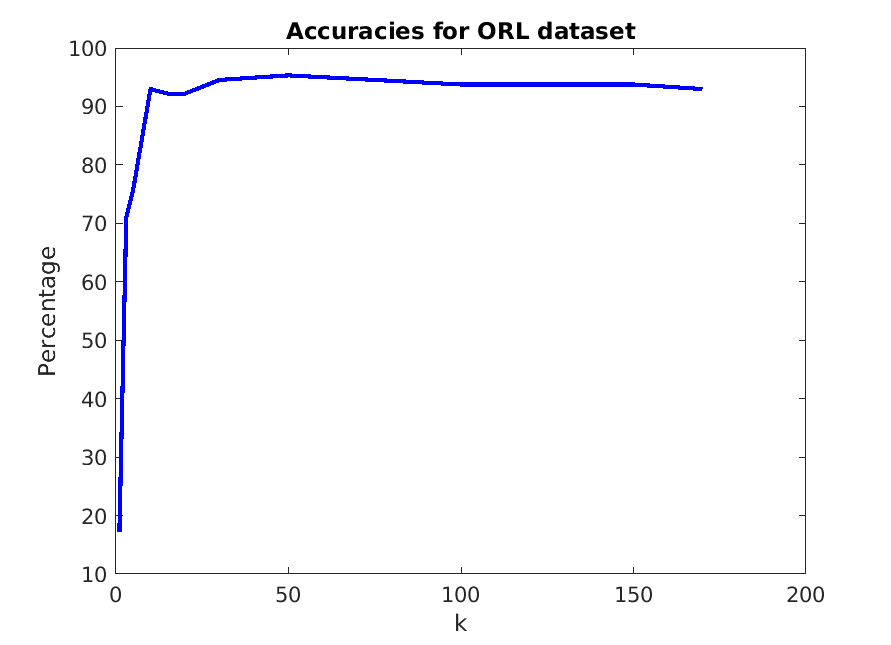
\includegraphics[width=1.34\textwidth]{orl.png}
    	\null\vspace*{-28pt}
    	\caption{Accuracy vs k}
	    \label{fig:4.1}
    \end{minipage} \\
\end{figure}
\vspace*{-24pt}
\subsubsection*{PCA using Eigenvector decomposition}
\quad In this section, we performed PCA by performing Eigenvector decomposition of the $L = \frac{1}{n-1}X^TX$ matrix using the matlab library function $eig$, where $X_{dxn}$ is the data matrix. \\
The results were exactly identical to the ones obtained in the previous part, since SVD of a matrix $X$ simply generates the eigenvectors of the matrices $X^TX$ and $XX^T$ (ie the left and right eigenvectors). the The maximum test accuracy of 95.31\% was obtained at k = 50.

\begin{figure}[h!]
    \centering
    \renewcommand{\thefigure}{4.1}
    \begin{minipage}[c][1\width]{0.4\textwidth}
    	\hspace*{-0.5in}
    	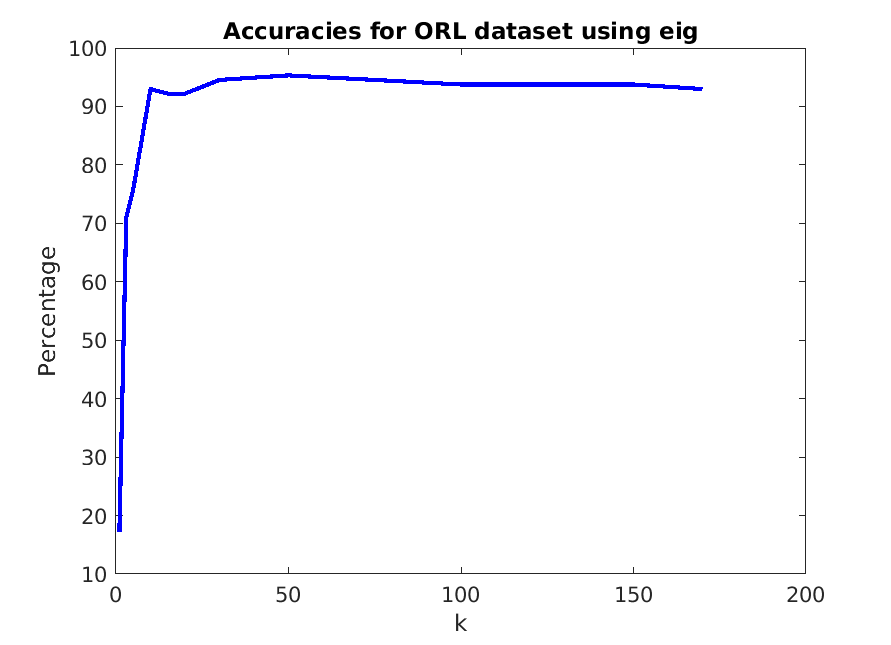
\includegraphics[width=1.34\textwidth]{orl_eig.png}
    	\null\vspace*{-28pt}
    	\caption{Accuracy v/s k}
	    \label{fig:4.1}
    \end{minipage} \\
\end{figure}

\newpage
\subsection*{4.2: Results on the Yale dataset}
\subsubsection*{Conventional PCA (Using all the top k eigenvectors)}
\quad Using the same method used in Part A of Section 4.1, we perform face recognition on the Yale Dataset. Since there is a huge contribution to the variance in the images arising from the lighting conditions, the eigenvectors corresponding to the highest variance are dominated by a variance in the lighting. Hence the accuracy obtained in this section is suboptimal. \\
The highest accuracy of 35.65\% was recorded for k = 1000.
\begin{figure}[h!]
    \centering
    \renewcommand{\thefigure}{4.1}
    \begin{minipage}[c][1\width]{0.4\textwidth}
    	\hspace*{-0.5in}
    	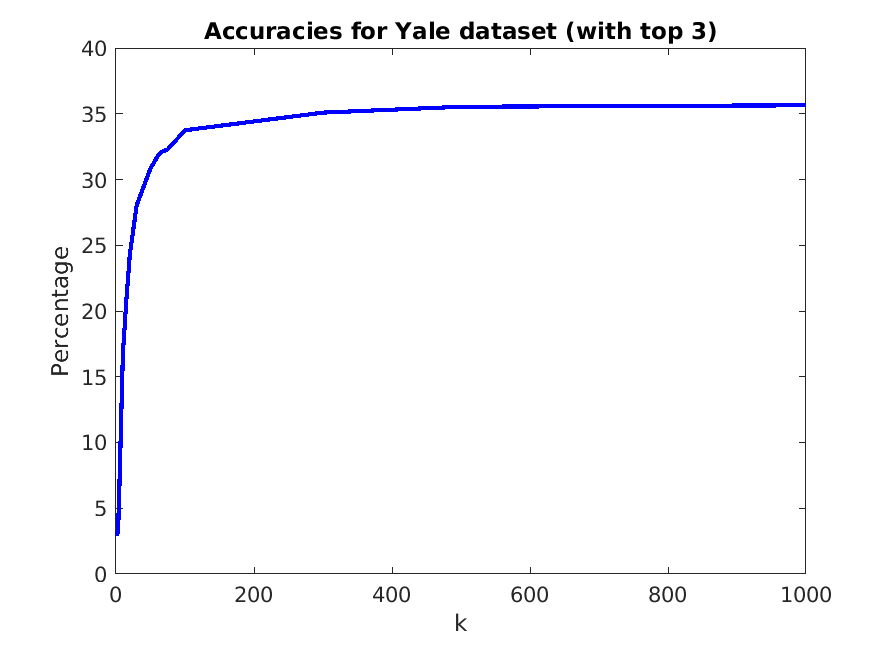
\includegraphics[width=1.34\textwidth]{yale.png}
    	\null\vspace*{-28pt}
    	\caption{Accuracy v/s k}
	    \label{fig:4.1}
    \end{minipage} \\
\end{figure}

\subsubsection*{PCA while ignoring the top 3 eigenvectors}
\quad As stated in the previous sub section, the first few eigenvectors are dominated by the variance arising due to lighting changes in the images. Hence to counter these effects, we ignore the top 3 eigenvectors, and recompute our accuracies. \\
The highest accuracy of 60.67\% was recorded for k = 1000.
\begin{figure}[h!]
    \centering
    \renewcommand{\thefigure}{4.1}
    \begin{minipage}[c][1\width]{0.4\textwidth}
    	\hspace*{-0.5in}
    	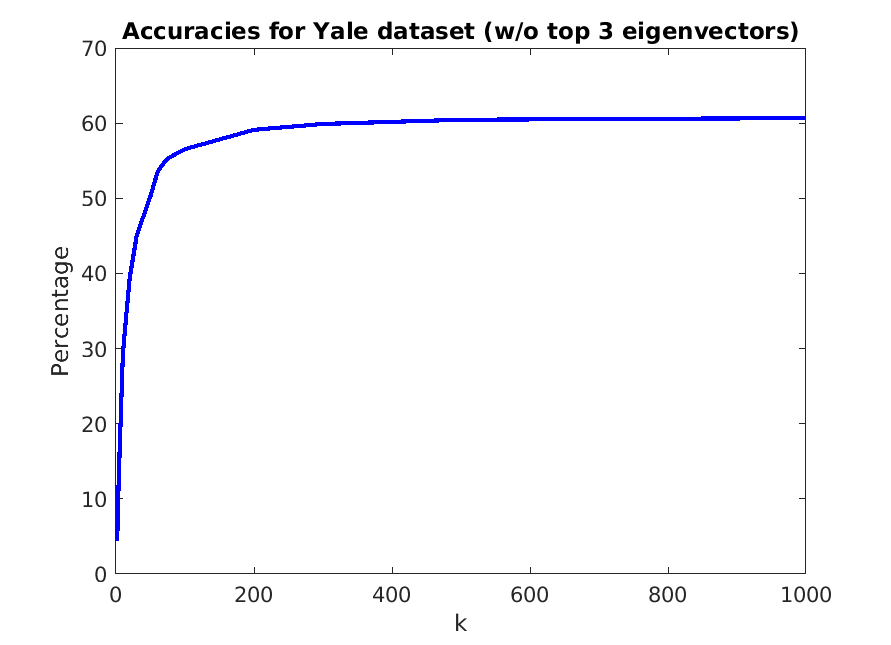
\includegraphics[width=1.34\textwidth]{yale_noptop3.png}
    	\null\vspace*{-28pt}
    	\caption{Accuracy v/s k}
	    \label{fig:4.1}
    \end{minipage} \\
\end{figure}

\newpage
\subsection*{4.3: Usage of code}
\begin{itemize}
\item Execute the \textbf{myMainScript.m} function to display the results and the plots. This takes around 68.22 seconds.
\item Since the dataset is being used for Q4, Q5, Q6 in the assignment, we have kept the datasets in a common directory just inside our submission directory. The ORL dataset is expected to be in a relative directory \textbf{'../../datasets/'}, and the Yale dataset is expected to be in a relative directory \textbf{'../../datasets/CroppedYale/'} \\ 
That is the per person directories should be as follows: \\\textbf{'../../datasets/ORL/s*/'} and \\\textbf{'../../datasets/CroppedYale/yaleB**/'}
\item The \textbf{loadOrl.m} and \textbf{loadYale.m} functions load the data.
\item The \textbf{fitPCA.m} and \textbf{fitPCAeig.m} functions generate the eigenvectors of the data matrix using the $svd$ and $eig$ functions respectively.
\item The \textbf{getPredictor.m} functions returns a struct which stores the relevant eigenvectors, and the subspace transformation operator using the said eigenvectors.
\item The \textbf{predict.m} function computes the test accuracy for a given data matrix, using the predictor object generated in the previous point.
\end{itemize}
\end{document}
